%
% @author   Shmish  "shmish90@gmail.com"
% @legal    MIT     "(c) Christopher Schmitt"
%


\documentclass{article}


%
% Document Imports
%

\usepackage{fancyhdr}
\usepackage{extramarks}
\usepackage{amsmath}
\usepackage{amssymb}
\usepackage{amsthm}
\usepackage{amsfonts}
\usepackage{algpseudocode}
\usepackage[table,xcdraw]{xcolor}
\usepackage{color}
\usepackage{tikz}
\usepackage{forest}
\usepackage{listings}
\usepackage{karnaugh-map}
\usepackage{graphicx}


\definecolor{dkgreen}{rgb}{0,0.6,0}
\definecolor{gray}{rgb}{0.5,0.5,0.5}
\definecolor{mauve}{rgb}{0.58,0,0.82}


\lstset{
  frame=tb,
  language=Verilog,
  aboveskip=3mm,
  belowskip=3mm,
  showstringspaces=false,
  columns=flexible,
  basicstyle=\ttfamily,
  numbers=none,
  numberstyle=\tiny\color{gray},
  keywordstyle=\color{blue},
  commentstyle=\color{dkgreen},
  stringstyle=\color{mauve},
  breaklines=true,
  breakatwhitespace=true,
  tabsize=3
}


%
% Document Configuation
%

\newcommand{\hwAuthor}{Christopher Schmitt}
\newcommand{\hwSubject}{CS 354}
\newcommand{\hwSection}{Section 02}
\newcommand{\hwSemester}{Fall 2019}
\newcommand{\hwAssignment}{Assignment 3}


%
% Document Enviornments
%

\setlength{\headheight}{65pt}
\pagestyle{fancy}
\lhead{\hwAuthor}
\rhead{
  \hwSubject \\
  \hwSection \\
  \hwSemester \\
  \hwAssignment
}

\newenvironment{problem}[1]{
  \nobreak\section*{Problem #1}
}{}


%
% Document Start
%

\begin{document}
  \begin{problem}{1}
    This simple CPU supports six opertions: AND, OR, ADD, SUB, SLT, and LI.
    This CPU has four registers available to it: \$0, \$1, \$2, and \$3.
    Instructions are loaded into the instruction register.  It should be
    noted that instructions can conform to two different formats, R-Type and
    L-Type, both of length nine.  R-Type instructions follow the form: Opcode
    (3 bits), Lhs (2 bits), Rhs (2 bits), and destination (2 bits).  L-Type
    instructions follow the form: Opcode (3 bits), Payload (4 bits), and
    destination (2 bits).  An Li decoder is used to in conjunction with several
    multiplexers to distingush between L-Type and R-Type instructions.  All of
    the actual operations are perfomed by the ALU, the rest of the CPU is simply
    moving and routing data around on the falling edge of each clock pulse.
    This data gets routed to the register file, which uses a register-select
    line to determine where the data on the write-data line should be routed.

    \begin{center}
      \lstinputlisting{src/CPU.v}
    \end{center}

    \begin{center}
      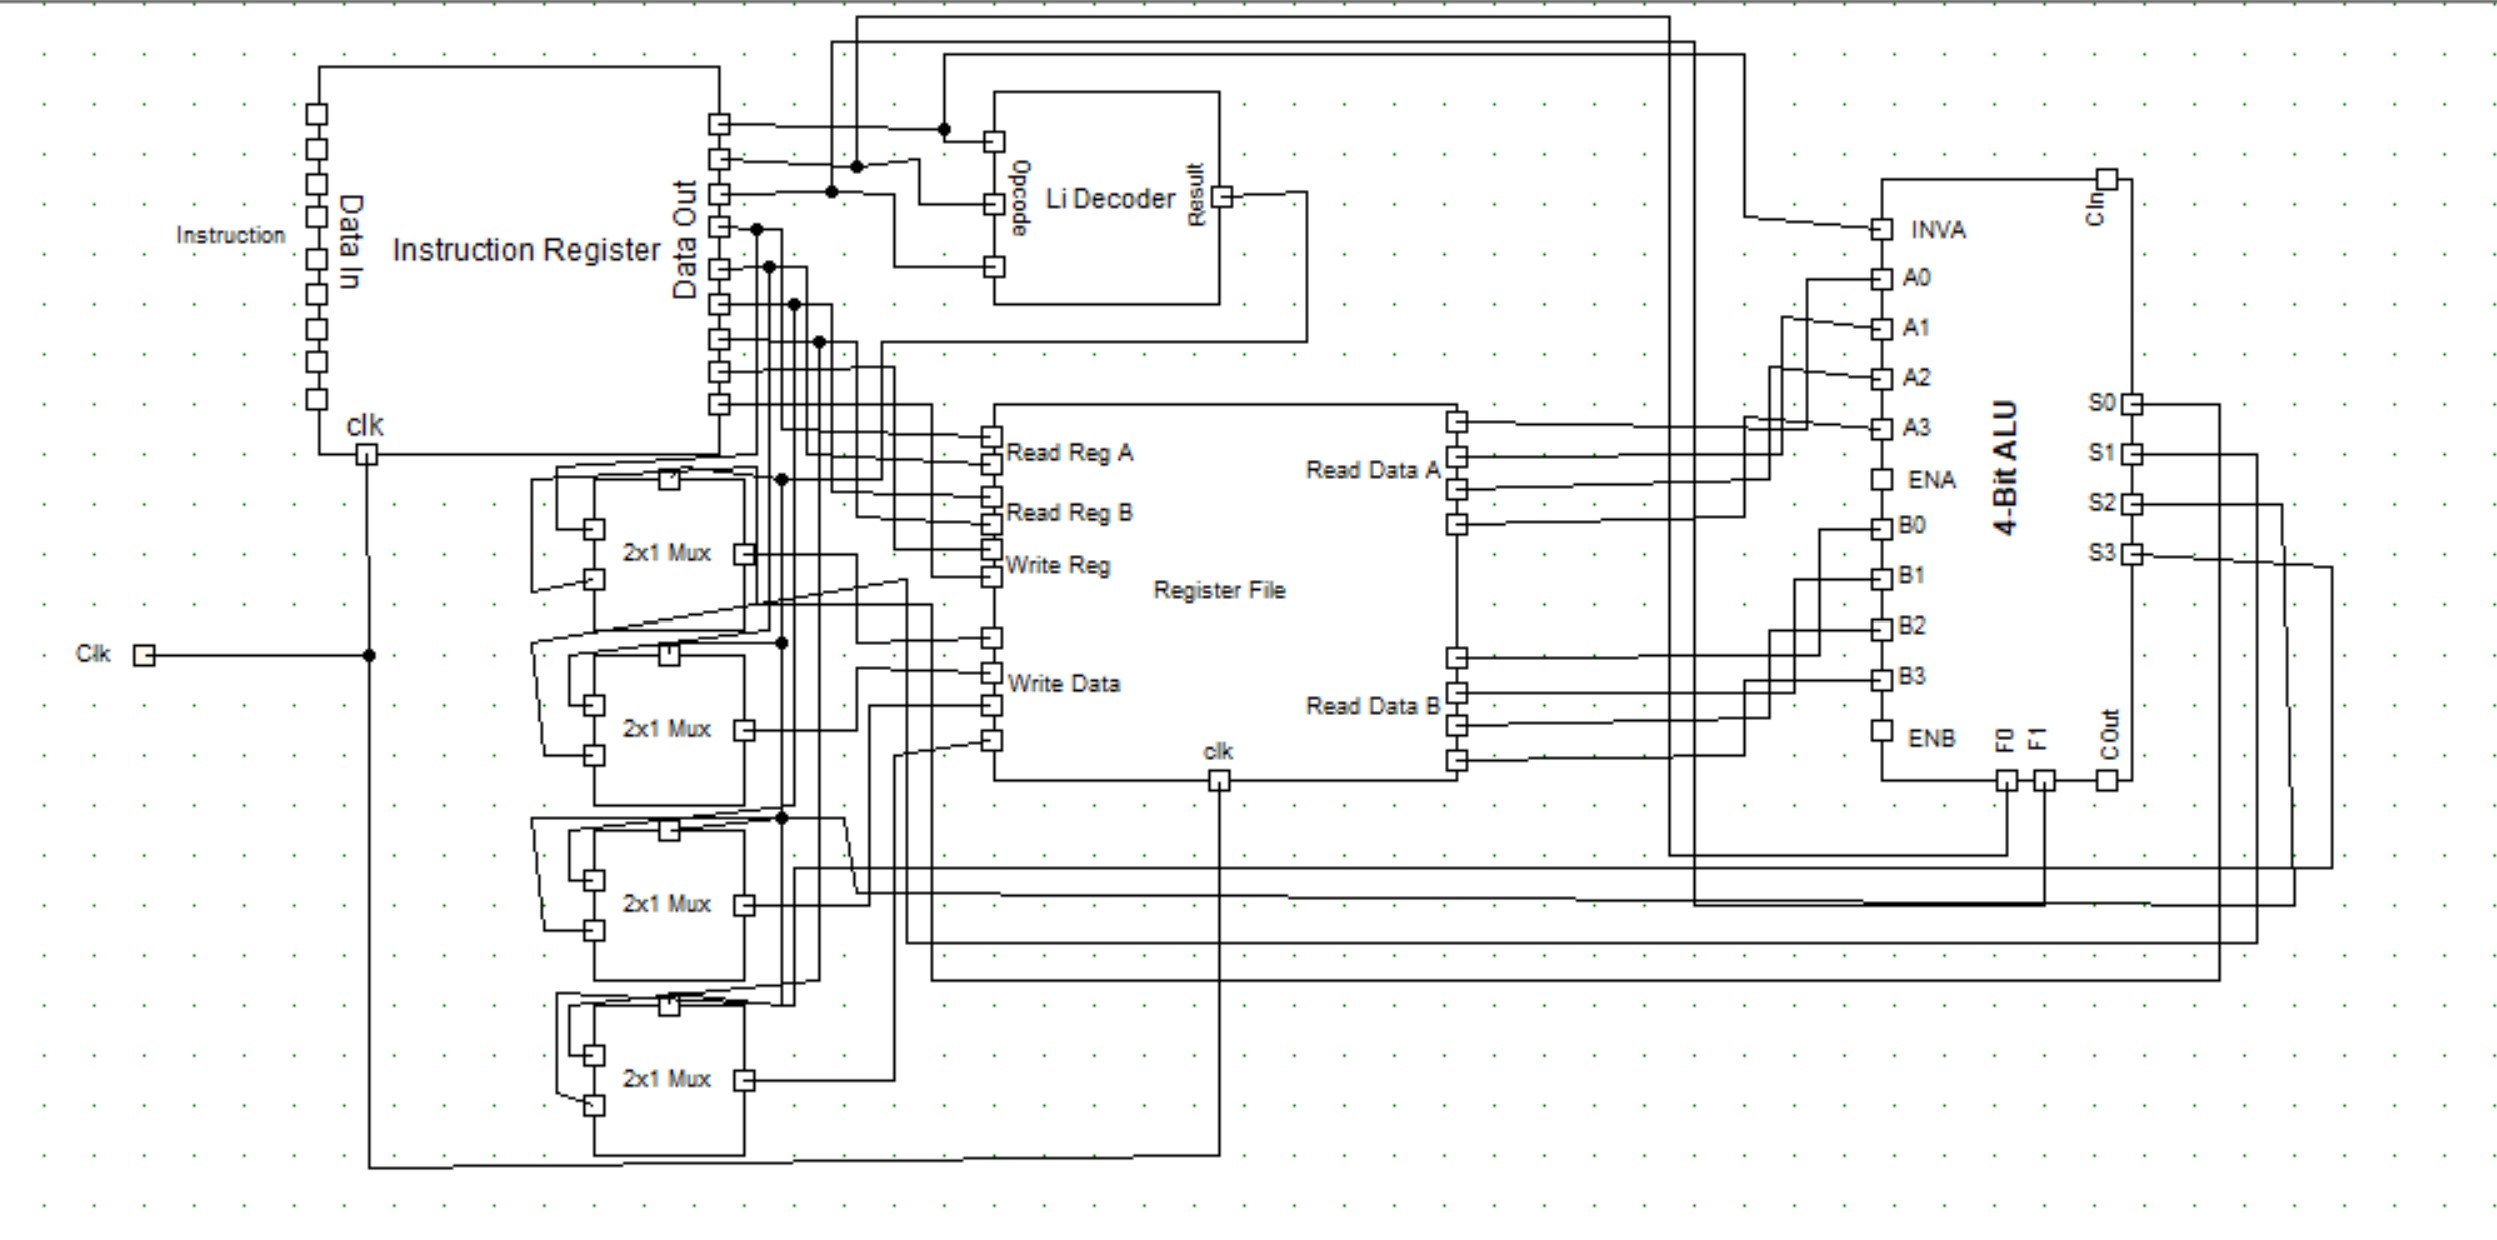
\includegraphics[scale=0.45]{images/CPU.jpg}
      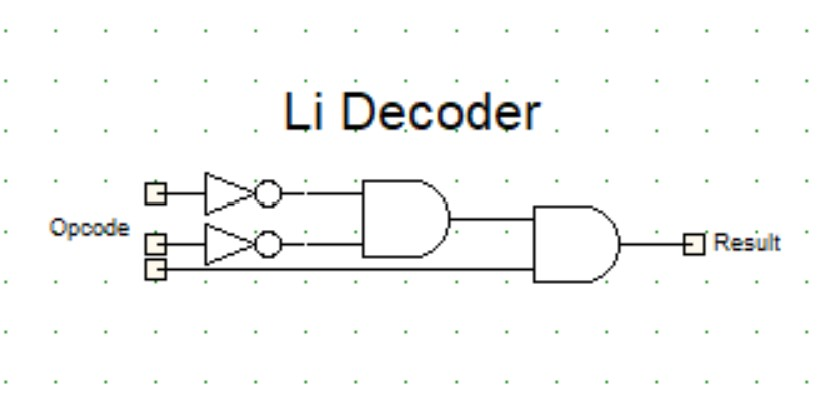
\includegraphics[scale=1]{images/LiDecoder.jpg}
      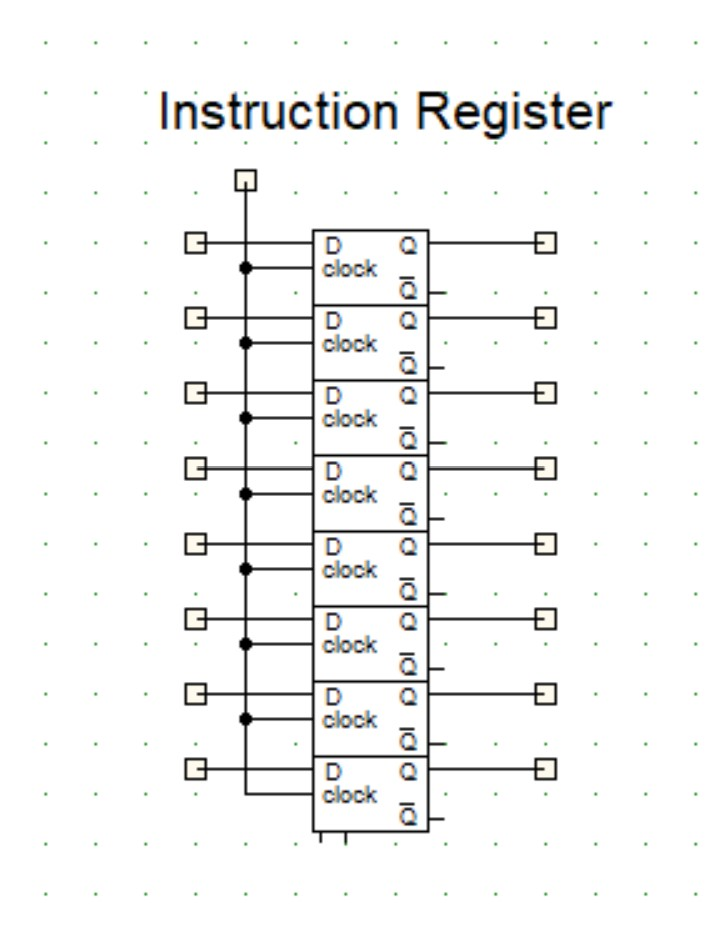
\includegraphics[scale=1]{images/InstructionRegister.jpg}
    \end{center}

    \begin{center}
      \begin{lstlisting}
        100111110     # Load 15 -> $2
        100100011     # Load 8 -> $3
        000101101     # $2 & $3 -> $1
        110011011     # $1 - $2 -> $3
        111110010     # SLT $2, $3, $0
        010101101     # $2 + $3 -> $1
        110000101     # $0 - $1 -> $1
        001011011     # $1 | $2 -> $3
      \end{lstlisting}
    \end{center}

    \begin{center}
      \begin{lstlisting}
        iverilog.exe ./CPU.v && vvp.exe a.out
        Instruction     WriteData
        xxxxxxxxx       xxxx  x
        100111110       xxxx  x
        100111110       1111 -1
        100100011       1111 -1
        100100011       1000 -8
        000101101       1000 -8
        000101101       1000 -8
        110011011       1000 -8
        110011011       1001 -7
        111110010       1001 -7
        111110010       0001  1
        010101101       0001  1
        010101101       1010 -6
        110000101       1010 -6
        110000101       0110  6
        001011011       0110  6
        001011011       0111  7
      \end{lstlisting}
    \end{center}
  \end{problem}
\end{document}